\documentclass[a4paper, amsfonts, amssymb, amsmath, reprint, showkeys, nofootinbib, twoside]{revtex4-1}
\usepackage[spanish]{babel}
\usepackage[utf8]{inputenc}
\usepackage{float}
\usepackage[colorinlistoftodos, color=green!40, prependcaption]{todonotes} \usepackage{amsthm} \usepackage{mathtools} \usepackage{physics}
\usepackage{xcolor}
\usepackage{graphicx}
\usepackage[left=23mm,right=13mm,top=35mm,columnsep=15pt]{geometry} 
\usepackage{adjustbox}
\usepackage{placeins}
\usepackage[T1]{fontenc}
\usepackage{lipsum}
\usepackage{csquotes}
\usepackage[normalem]{ulem}
\usepackage{tikz}
\usepackage{circuitikz}
\useunder{\uline}{\ul}{}
\usepackage[pdftex, pdftitle={Article}, pdfauthor={Author}]{hyperref} % For hyperlinks in the PDF
%\setlength{\marginparwidth}{2.5cm}
\bibliographystyle{apsrev4-1}

\begin{document}

%El título del experimento realizado es importante.
\title{Arduino y Ley de Ohm. Manejo de Multimetro}


\author{Sergio Montoya Ramirez}
\email[Correo institucional: ]{s.montoyar2@uniandes.edu.co}

%Si necesitan poner un segundo autor, deben eliminar los porcentajes (%) iniciales.
  
%\author{Second Author}
%\email{Second.Author@institution.edu}

\affiliation{Universidad de los Andes, Bogotá, Colombia.}

\date{\today} % Si lo dejan vacío no les saldrá fecha. La fecha que se muestra es del día en que se compila.

\begin{abstract}

  Este texto es el preinforme de la sesión 2 del experimento 2 del curso Electronica para Ciencias de la Universidad de los Andes durante el semestre 202310. Tiene como objetivo la preparación para el posterior desarrollo de la sesión previamente enunciada.

\end{abstract}

\maketitle

\section{Resistencias Equivalentes}

Realice el calculo detallado de las resistencia equivalente entre los puntos $A$ y $B$ para cada uno de los circuitos de las figuras \ref{fig:circuito_1}, \ref{fig:circuito_2}, \ref{fig:circuito_3}

Antes de realizar cualquiera de estos ejercicios considero relevante dar a conocer la fuente de mi información y revlar el metodo que seguiremos para encontrar la respuesta. En particular utilizaremos la diapositiva $25$ de \textit{Diapositivas 1: Fundamentos de Circuitos} que son las diapositivas guia del curso. En particular la información ahi dada es:
\begin{enumerate}
  \item \textbf{Resistencias en Serie: } Una serie $R_1,R_2,\ldots,R_n$ de resistencias en serie pueden ser reemplazadas por una resistencia $R_s$ tal que:
  \begin{equation}
    R_s = \sum_{i=1}^{n} R_i \label{eq:Rs} \end{equation}
\item \textbf{Resistencias en Paralelo: } Una serie $R_1,R_2,\ldots,R_n$ de resistencias en paralelos pueden ser remplazadas por una resistencia $R_p$ tal que: 
  \begin{equation}
    \frac{1}{R_p}=\sum_{i=1}^{n} \frac{1}{R_i} \label{eq:Rp}
  \end{equation}
\end{enumerate}

Con esta información va a ser suficiente para solucionar todos estos ejercicios.

\begin{figure}[H]
  \centering
  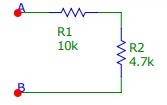
\includegraphics[width=0.4\textwidth]{Graficas/circuito_1.jpeg}
  \caption{Grafica de resistencias en serie}
  \label{fig:circuito_1}
\end{figure}

En este caso, tenemos un circuito con dos resistencias en serie una de $10$ kilo ohmnios y otra de $4.7$ kilo ohmnios. Por lo tanto solo debemos aplicar la ecuación \ref{eq:Rs} para allar la respuesta que en este caso es:
\begin{align*}
  R_s &= \sum_{i=1}^{n} R_i \\
  &= 10k \Omega+ 4.7k \Omega\\
  R_s &= 14.7k \Omega\\
.\end{align*}

\begin{figure}[H]
  \centering
  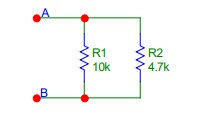
\includegraphics[width=0.4\textwidth]{Graficas/circuito_2.jpeg}
  \caption{Grafica de resistencias en paralelo}
  \label{fig:circuito_2}
\end{figure}

En este caso, tenemos un circuito con dos resistencias en paralelo una de $10$ kilo ohmnios y otra de $4.7$ kilo ohmnios. Por lo tanto solo debemos aplicar la ecuación \ref{eq:Rp} para encontrar la respuesta que en esta caso es:
\begin{align*}
  \frac{1}{R_p}&= \sum_{i=1}^{n} \frac{1}{R_i} \\
  &= \frac{1}{10k\Omega}+\frac{1}{4.7k\Omega} \\
  &= \frac{10k\Omega + 4.7k\Omega}{47k^2\Omega^2} \\
  &= \frac{14.7k\Omega}{47k^2\Omega^2} \\
  \frac{1}{R_p} &= \frac{14.7}{47k\Omega} \\
  R_p &= \frac{47k\Omega}{14.7} \\
  R_p &\approx 3.19728 \\
.\end{align*}

\begin{figure}[H]
  \centering
  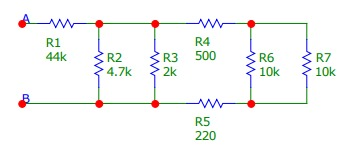
\includegraphics[width=0.4\textwidth]{Graficas/circuito_3.jpeg}
  \caption{Circuito de resistencias en formación mixta.}
  \label{fig:circuito_3}
\end{figure}

En este caso, vamos a tener que realizar una reducción por pasos aprovechando la equivalencia de cierto grupo de Resistencias. Para iniciar aprovecharemos la equivalencia de las resistencias $2$ y $3$ (que estan en paralelo) y $6$ y $7$ (que tambien estan en paralelo). Dada la facilidad de los calculos y que ya los presentamos en puntos anteriores en esta ocasión no los mostraremos en favor de desarrollar el circuito. Luego de hacer los calculos el circuito quedaria:

\begin{figure}[h!]
  \begin{center}
    \begin{circuitikz}
      \draw (0,0)
      to[V,v=$U_q$] (0,2) % The voltage source
      to[R=$R_1\ 44k$] (2,2)
      to[R=$R_{2,3}\ 1.40k$] (2,0) % The resistor
      to[short] (0,0);
      \draw (2,2)
      to[R=$R_4\ 500$] (4,2)
      to[R=$R_{6,7}\ 5k$] (4,0)
      to[R=$R_5\ 220$] (2,0);
   \end{circuitikz}
    \caption{Circuito en donde reemplazamos las equivalencias de $R_2$ y $R_3$ asi como de $R_6$ y $R_7$}
  \end{center}
\end{figure}

Ahora con esto podemos notar que los circuitos $R_4$, $R_{6,7}$ y $R_{5}$ estan en serie. Por lo que los podemos poner la equivalencia de todos en una sola con la ecuacion \ref{eq:Rs}. Con esto quedaria como:

\begin{figure}[h!]
  \begin{center}
    \begin{circuitikz}
      \draw (0,0)
      to[V,v=$U_q$] (0,2) % The voltage source
      to[R=$R_1\ 44k$] (2,2)
      to[R=$R_{2,3}\ 1.40k$] (2,0) % The resistor
      to[short] (0,0);
      \draw (2,2)
      to[short] (4,2)
      to[R=$R_{4\to7}\ 5.72k$] (4,0)
      to[short] (2,0);
   \end{circuitikz}
    \caption{Circuito en donde reemplazamos las equivalencias de $R_4$, $R_5$ y $R_{6,7}$}
  \end{center}
\end{figure}

Ahora con esto solo nos quedara encontrar la equivalencia entre $R_{2,3}$ y $R_{4\to7}$ que dado que estan en paralelo nos queda como

\begin{figure}[h!]
  \begin{center}
    \begin{circuitikz}
      \draw (0,0)
      to[V,v=$U_q$] (0,2) % The voltage source
      to[R=$R_1\ 44k$] (2,2)
      to[R=$R_{2\to7}\ 1.12k$] (2,0) % The resistor
      to[short] (0,0);
   \end{circuitikz}
    \caption{Circuito en donde reemplazamos las equivalencias de $R_{2,3}$ y $R_{4\to7}$}
  \end{center}
\end{figure}

Con esto entonces caemos en esencia en el mismo punto que la imagen \ref{fig:circuito_1} y por lo tanto podemos simplemente sumamos ambos y nos queda como resultado $45.12k\Omega$. Considero importante aclarar que para la realización de los diagramas segui el tutorial disponible de este link: \url{https://latex-tutorial.com/tutorials/circuitikz/}

\section{Propagación de Error}

Considere usará resistencias comerciales con tolerancia $5\%$. Asuma que sus valores tienen una distribución normal, con tolerancia igual a tres desviación estandar, es decir asuma  $3\sigma_R=0.05R$

Mediante propagación de errores, estime la tolerancia de la resistencia equivalente para los circuitos de las figuras \ref{fig:circuito_1} y \ref{fig:circuito_2}

\begin{enumerate}
  \item Dado que tenemos un circuito en serie de dos componentes entonces el error seria:
    \begin{align*}
      \sigma_{R_1}&= \frac{0.05\cdot R_1}{3} \\
      \sigma_{R_2}&= \frac{0.05\cdot R_2}{3} \\
      \frac{\partial R_{eqv}}{\partial R_{1}} &= 1 \\
      \frac{\partial R_{eqv}}{\partial R_{2}} &= 1 \\
      \sigma_{R_{eqv}}&= \sqrt{\left( \frac{0.05R_1}{3} \right)^2 + \left( \frac{0.05 R_2}{3} \right)^2}  \\
      &= \frac{0.05}{3}\sqrt{R_1^2+R_2^2}  \\
      &= 0.18k \\
    .\end{align*}
  \item Dado que tenemos un circuito en paralelo de dos componentes entonces el error seria:
    \begin{align*}
      \sigma_{R_1}&= \frac{0.05\cdot R_1}{3} \\
      \sigma_{R_2}&= \frac{0.05\cdot R_2}{3} \\
      \frac{\partial R_{eqv}}{\partial R_{1}} &= \frac{R_2^2}{\left( R_1+R_2 \right)^2}	 \\
      \frac{\partial R_{eqv}}{\partial R_{2}} &= \frac{R_1^2}{\left( R_1+R_2 \right)^2} \\
      \sigma_{R_{eqv}}&= \sqrt{\left( \left( \frac{R_2^2}{\left( R_1+R_2 \right)^2} \right) \frac{0.05R_1}{3} \right)^2}\\
      &+\left( \frac{R_1}{\left( R_1+R_2 \right)^2}\frac{0.05R_2}{3} \right)^2  \\
      &= \sqrt{\left( \frac{2\cdot 0.05R_1R_2}{3\left( R_1+R_2 \right)^2} \right)^2}  \\ 
      &= 7.09k \\
    .\end{align*}
\end{enumerate}

\section{Potencia Disipada}

Calcule la potencia disipada por una resistencia $R$ conectada a una fuente de $5V$. Asuma
\begin{enumerate}
  \item $R=1\Omega$ 
  \item $R=10\Omega$ 
  \item $R=100\Omega$ 
\end{enumerate}

Antes de resolver este ejercicio considero importante hablar de la fuente y la información que utilizaremos para solucionar este problema. Para solucionar este punto utilizaremos la diapositiva 27 de \textit{Diapositiva 1: Fundamentos de Circuitos} la cual da como información un par de formulas para la potencia disipada por un resorte. Aunque en esta diapositiva dan dos ecuaciones considero que la mas relevante (bajo las condiciones dadas previamente) es
\begin{equation}
  P = \frac{V^2}{R} \label{Pr}
\end{equation}

Ya con esto es suficiente para conseguir la potencia disipada y simplemente dividimos $V^2=25V^2$ por la resistencia lo que nos da:
\begin{enumerate}
  \item $\left( 1\Omega \right) \frac{25V^2}{1\Omega}=25$
  \item $\left( 10\Omega \right) \frac{25V^2}{10\Omega}=2.5$ 
  \item $\left( 100\Omega \right) \frac{25V^2}{100\Omega}=0.25$
\end{enumerate}

\section{Precio de Resistencias}

Los precios aqui enunciados fueron obtenidos por mercado libre dado que no me encontraba en la ciudad al momento de realizar este informe. En particular obtuve que:
\begin{enumerate}
  \item $1$ W: $4\times 6.000$ 
  \item $\frac{1}{4}$ W: $10\times 6000$ 
  \item $\frac{1}{2}$ W: $5\times 6000$
  \item $5$ W: $1\times 4235$
\end{enumerate}
\bibliographystyle{abbrv}
\bibliography{Referencias}
\end{document}
